% Auto-generated by scripts/build_eval_figures.py — do not edit.
\begin{figure}[t]
  \centering
  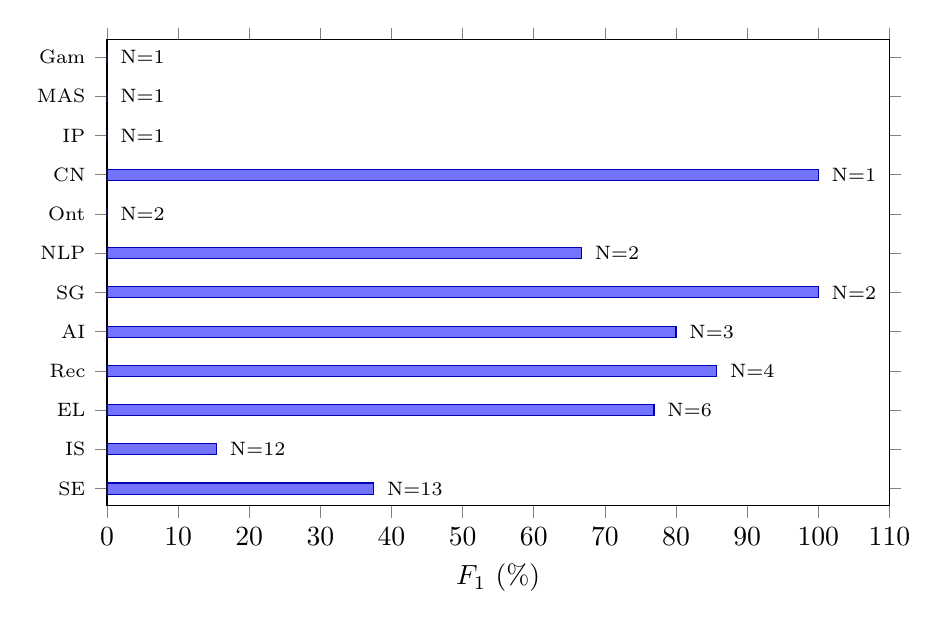
\begin{tikzpicture}
    \begin{axis}[
      width=0.95\linewidth, height=7.5cm,
      xbar, xmin=0, xmax=110,
      bar width=4pt, enlarge y limits=0.04,
      xlabel={$F_1$ (\%)},
      ytick={0,1,2,3,4,5,6,7,8,9,10,11},
      yticklabels={SE,IS,EL,Rec,AI,SG,NLP,Ont,CN,IP,MAS,Gam},
      yticklabel style={font=\scriptsize},
      tick align=outside,
      nodes near coords style={font=\tiny},
      ]
      \addplot+[fill=blue!55,draw=blue!70!black] coordinates {(37.5,0) (15.4,1) (76.9,2) (85.7,3) (80.0,4) (100.0,5) (66.7,6) (0.0,7) (100.0,8) (0.0,9) (0.0,10) (0.0,11)};
      \node[anchor=west,font=\scriptsize] at (axis cs:37.5,0) { \,N{=}13 };
      \node[anchor=west,font=\scriptsize] at (axis cs:15.4,1) { \,N{=}12 };
      \node[anchor=west,font=\scriptsize] at (axis cs:76.9,2) { \,N{=}6 };
      \node[anchor=west,font=\scriptsize] at (axis cs:85.7,3) { \,N{=}4 };
      \node[anchor=west,font=\scriptsize] at (axis cs:80.0,4) { \,N{=}3 };
      \node[anchor=west,font=\scriptsize] at (axis cs:100.0,5) { \,N{=}2 };
      \node[anchor=west,font=\scriptsize] at (axis cs:66.7,6) { \,N{=}2 };
      \node[anchor=west,font=\scriptsize] at (axis cs:0.0,7) { \,N{=}2 };
      \node[anchor=west,font=\scriptsize] at (axis cs:100.0,8) { \,N{=}1 };
      \node[anchor=west,font=\scriptsize] at (axis cs:0.0,9) { \,N{=}1 };
      \node[anchor=west,font=\scriptsize] at (axis cs:0.0,10) { \,N{=}1 };
      \node[anchor=west,font=\scriptsize] at (axis cs:0.0,11) { \,N{=}1 };
    \end{axis}
  \end{tikzpicture}
  \caption{Per-class $F_1$ (\%) of \texttt{qwen2.5:14b-instruct} on the gold set, sorted by gold support (annotated next to each bar). Classes whose support is one or two collapse to $F_1{=}0$ and pull the macro average down.}
  \label{fig:per-class-f1}
\end{figure}
